\documentclass[11pt]{article}
\usepackage[a4paper,margin=1.05in]{geometry}
\usepackage{amsmath,amssymb,amsthm}
\usepackage{booktabs,array,graphicx,xcolor,enumitem,longtable}
\usepackage[colorlinks=true,linkcolor=blue!50!black,urlcolor=blue!50!black,citecolor=blue!50!black]{hyperref}
\usepackage{caption}
\captionsetup{font=small,labelfont=bf}
\newcommand{\TabN}{500}
\newcommand{\MeanSq}{4.052}
\newcommand{\KSq}{20000}
\newcommand{\QDirect}{85}
\newcommand{\MeanDirect}{4.3747}
\newcommand{\QWrap}{45}
\newcommand{\MeanWrap}{6.915}
\newcommand{\TotalCases}{337995}
\newcommand{\VerSha}{d2f57b990c511d7f}
\newcommand{\Bnum}{97}
\newcommand{\Bden}{562}
\newcommand{\FirstFive}{23,\,28,\,36,\,40,\,43,\,47}
\newcommand{\CountFive}{94}

\newtheorem{theorem}{Theorem}[section]
\newtheorem{lemma}[theorem]{Lemma}
\newtheorem{proposition}[theorem]{Proposition}
\newtheorem{corollary}[theorem]{Corollary}
\theoremstyle{definition}
\newtheorem{definition}[theorem]{Definition}
\newtheorem{remark}[theorem]{Remark}
\newcommand{\N}{\mathbb{N}}
\newcommand{\dist}{\operatorname{d}}
\newcommand{\RDY}{\mathsf{READY}}

\title{\textbf{Squares and Power Sequences in the Reversible\\ Square-Multiplication Graph}\\[4pt]
\large UNNS-U2-SQ \,--\, version 1.0 (v001)}
\author{UNNS Research Collective}
\date{9 November 2026}

\begin{document}
\maketitle

\begin{abstract}
\noindent Let $G$ be the graph on the positive integers in which $kN$ is joined to $k(N+1)^2$ for all $k,N\ge1$, and let $\dist$ be its graph distance.
We prove that consecutive squares are at distance at most $5$ and that $5$ is attained:
$\sup_{n\ge1}\dist(n^2,(n+1)^2)=5$. The upper bound comes from $24$ explicit path identities, one for each residue class of $n$ modulo $24$; in each class
the path from $n^2$ to $(n+1)^2$ has at most five edges, its labels are polynomials in a class parameter, and every step is certified by an integral positive cofactor.
The lower bound is the disjointness of the radius-two balls around $23^2=529$ and $24^2=576$. More generally, an edge $x\!-\!y$ lifts to a chain
$x^k,x^{k-1}y,\dots,y^k$ of $k$ edges, so $\dist(x^k,y^k)\le k\,\dist(x,y)$ and $\dist(n^k,(n+1)^k)\le 6k$. The path identities have strictly increasing polynomial intermediate states,
so the parameter can be read back from the current integer; this yields deterministic finite-control selectors with no external input that pass through
$1^2,2^2,3^2,\dots$ with at most five moves per square, and through $1^k,2^k,3^k,\dots$ with at most $6k$ moves per power.
\end{abstract}

\section{Introduction}\label{sec:intro}
\paragraph{Provenance.} The graph $G$ is the undirected closure of the SELECT-II transformation $m\mapsto m(N+1)^2/N$ ($N\mid m$) of the UNNS Substrate.
Its uniform successor bound $\dist(n,n+1)\le6$ is established in UNNS-U1-BND~\cite{u1bnd}, and the finite-control successor selector (43 control states)
in UNNS-U2-001~\cite{u2}. Both releases, the earlier notes~\cite{u0,u1} and the frozen reference collection~\cite{gig,repo} are left unchanged. The present release is the
separate UNNS-U2-SQ baseline for squares and power sequences.

\paragraph{Question.} Powers $n^k$ are the simplest algebraic progressions after the integers themselves. The successor selector of~\cite{u2} gives a route from $n-1$ to $n$
in at most six moves; how far apart are $n^2$ and $(n+1)^2$ really, and can a fixed rule with no external input choose the path?

\begin{theorem}[Summary]\label{thm:summary}
\begin{enumerate}[label=(\alph*),nosep]
\item $\dist(n^2,(n+1)^2)\le5$ for all $n\ge1$, and $\dist(23^2,24^2)=5$; hence $\sup_n\dist(n^2,(n+1)^2)=5$.
\item For adjacent or arbitrary $x,y$ and $k\ge1$, $\dist(x^k,y^k)\le k\,\dist(x,y)$; in particular $\dist(n^k,(n+1)^k)\le6k$. Also $\dist(n^2,(n+1)^2)\le8$ by a short argument not using (a).
\item There is a deterministic selector with $\QDirect$ control states, reading only the current integer, that returns to its ready state exactly at $1^2,2^2,3^2,\dots$ with at most five moves between consecutive squares.
There is also a $\QWrap$-state selector doing the same in at most eight moves, built on the successor selector of~\cite{u2}. For each fixed $k$ a finite-control selector realizes $1^k,2^k,3^k,\dots$ in at most $6k$ moves per step.
\end{enumerate}
\end{theorem}

\section{Preliminaries}\label{sec:prelim}
A move $+N$ from $x$ requires $N\mid x$ and gives $x(N+1)^2/N$; a move $-N$ requires $(N+1)^2\mid x$ and gives $xN/(N+1)^2$. These are mutually inverse and the edges of $G$ are exactly the pairs they join.

\begin{lemma}[Scaling]\label{lem:scale}
If $\{x,y\}$ is an edge, so is $\{mx,my\}$ for every $m\ge1$. Hence $\dist(ma,mb)\le\dist(a,b)$.
\end{lemma}
\begin{proof} Multiply the cofactor $k$ in $x=kN$, $y=k(N+1)^2$ by $m$. \end{proof}

\begin{lemma}[Power lifting]\label{lem:lift}
For $k\ge1$ and any $x,y$: $\dist(x^k,y^k)\le k\,\dist(x,y)$. For an edge $\{x,y\}$ the chain
$x^k,\,x^{k-1}y,\,\dots,\,y^k$ is a path of $k$ edges in which every step carries the label of the original edge.
\end{lemma}
\begin{proof} Consecutive terms are $x^{k-j}y^{j}=m\,x$ and $x^{k-j-1}y^{j+1}=m\,y$ with $m=x^{k-j-1}y^j$, an edge by Lemma~\ref{lem:scale}; write $x=cN$, $y=c(N+1)^2$ and the move is $+N$ with cofactor $mc$.
Apply this along a shortest path from $x$ to $y$. \end{proof}
\begin{corollary}\label{cor:6k} $\dist(n^k,(n+1)^k)\le 6k$; in particular $\dist(n^2,(n+1)^2)\le12$, by $\dist(n,n+1)\le6$~\cite{u1bnd}. \end{corollary}

\begin{lemma}[Square-specific route]\label{lem:sq8}
For $n\ge2$, $n^2\xrightarrow{-(n-1)}n-1$ and $n\xrightarrow{+n}(n+1)^2$ are legal moves. Hence $\dist(n^2,(n+1)^2)\le 1+\dist(n-1,n)+1\le8$.
\end{lemma}
\begin{proof} $(n-1+1)^2=n^2$ divides $n^2$ and $n^2(n-1)/n^2=n-1$; and $n\mid n$ with $n(n+1)^2/n=(n+1)^2$. For $n=1$, $1\to4$ is an edge. \end{proof}

\section{The exact constant}\label{sec:main}
\begin{theorem}\label{thm:main}
$\sup_{n\ge1}\dist(n^2,(n+1)^2)=5$.
\end{theorem}

\subsection{Upper bound: 24 path identities}
Write $n=24t+r$ with $0\le r<24$. For each $r$ Appendix~\ref{app:ids} gives at most five signed labels $N_1(t),\dots,N_\ell(t)$, $\ell\le5$, polynomials in $t$.
\begin{lemma}[Certificates]\label{lem:cert}
For each $r$ and all integers $t\ge t_0(r)$ the labelled path starting at $n^2$ is legal at every step and ends at $(n+1)^2$.
\end{lemma}
\begin{proof} Compose the moves symbolically. At each step the current state equals $c\cdot N$ (forward) or $c\,(N+1)^2$ (inverse) with a cofactor $c(t)$; the verifier checks by exact polynomial division
that $c(t)$ is a polynomial, integer valued, and at least $1$ for $t\ge t_0$ (all coefficients nonnegative after shifting $t\mapsto t_0+u$ and value $\ge1$ at $u=0$), and that the labels are integer valued and positive; the final state is $(n+1)^2$ as a polynomial identity.
All $24$ certificates pass (check Q1 of Table~\ref{tab:status}). \end{proof}
\begin{remark}[Example] For $n=24t+1$ the states are
\begin{align*}
(24t{+}1)^2&\xrightarrow{+(24t+1)^2}4(288t^2{+}24t{+}1)^2\xrightarrow{-24t(12t+1)}96t(12t{+}1)\\
&\xrightarrow{+6t}16(6t{+}1)^2(12t{+}1)\xrightarrow{-(12t+1)}4(12t{+}1)^2=(n+1)^2.
\end{align*}
\end{remark}
Only $n\in\{1,2,3\}$ lie below $t_0$ in their classes; for these the paths $1\to4$, $4\to16\to100\to9$ and $9\to100\to16$ are listed in the data file and verified. Hence $\dist(n^2,(n+1)^2)\le5$ for all $n$.

\subsection{Lower bound}
\begin{lemma}\label{lem:lower} $\dist(23^2,24^2)=5$. \end{lemma}
\begin{proof} The radius-two balls $B_2(529)$ and $B_2(576)$ have $\Bnum$ and $\Bden$ vertices and are disjoint, computed by two independent neighbour-enumeration programs; so no path of length $\le4$ exists. The path
$529\to280900\to1056\to13824\to3072\to576$ with moves $+529,-264,+11,-2,-3$ has length five. \end{proof}
This proves Theorem~\ref{thm:main}. The lower bound is a computation; the exact distance table for $n\le\TabN$ shows the value $5$ for $\CountFive$ values of $n$, the first being $\FirstFive$. Whether $5$ occurs for infinitely many $n$ is open.

\begin{figure}[ht]\centering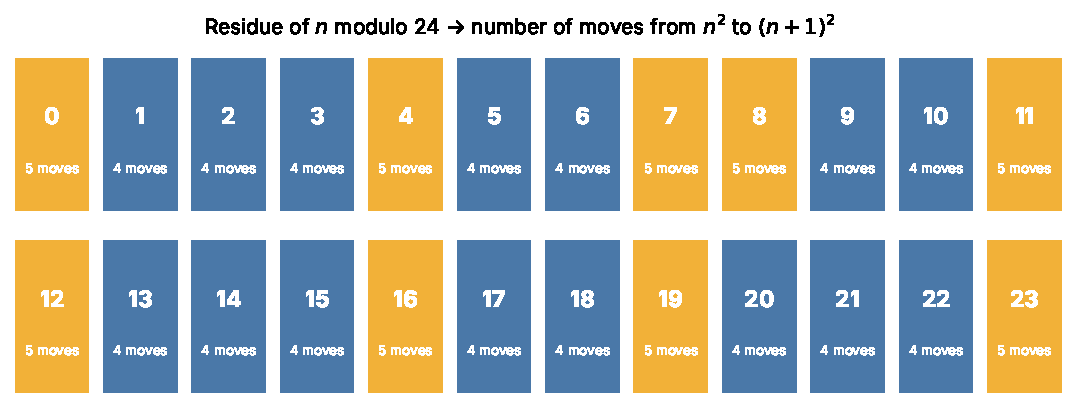
\includegraphics[width=.9\textwidth]{figures/fig1_residue_cover.pdf}
\caption{The 24 residue classes and the number of moves of their identity (at most five).}\end{figure}
\begin{figure}[ht]\centering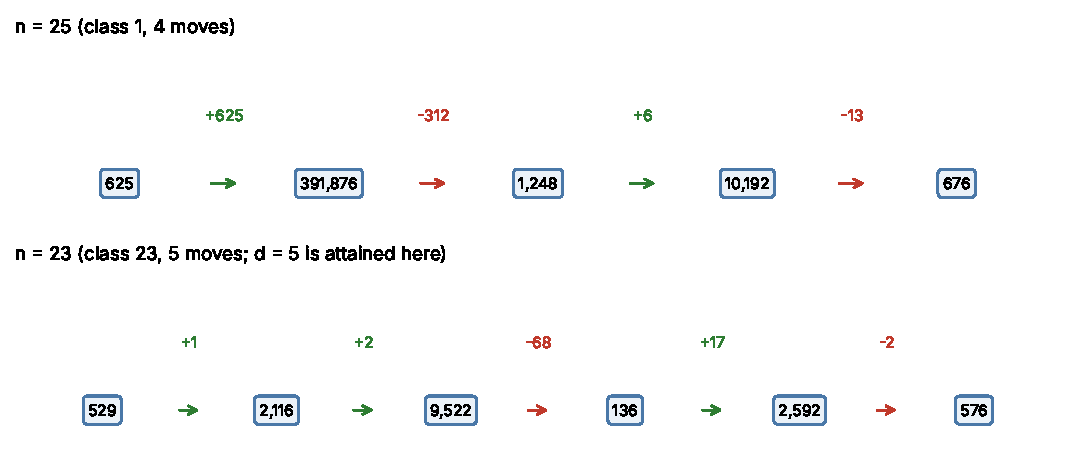
\includegraphics[width=.9\textwidth]{figures/fig3_example_paths.pdf}
\caption{Two paths from $n^2$ to $(n+1)^2$ generated by the identities (green: forward move $+N$, red: inverse move $-N$).}\end{figure}
\begin{figure}[ht]\centering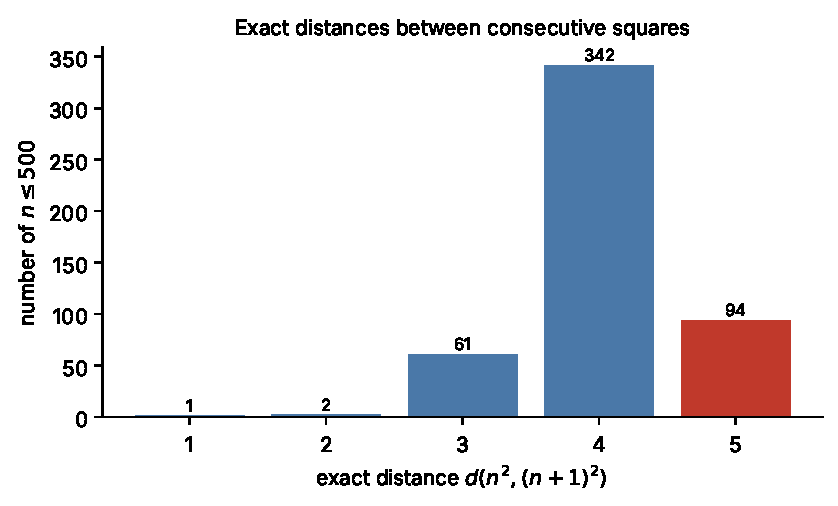
\includegraphics[width=.68\textwidth]{figures/fig2_distribution.pdf}
\caption{Exact distances between consecutive squares for $n\le\TabN$ (mean $\MeanSq$); the identities do not always give the shortest path but never exceed five moves.}\end{figure}
\begin{center}\begin{tabular}{rr}\toprule distance $d(n^2,(n+1)^2)$ & number of $n\le\TabN$\\\midrule
1 & 1 \\
2 & 2 \\
3 & 61 \\
4 & 342 \\
5 & 94 \\
\bottomrule\end{tabular}
\end{center}

\section{Finite-control generation of squares and powers}\label{sec:select}
We use the selector model of~\cite{u2}: a finite set of control states, a distinguished ready state, and a move rule reading exact arithmetic on the current integer and the control state only; no target, counter or other external datum.

\begin{lemma}[Recoverability]\label{lem:recover}
In each of the 24 identities the states $s_0(t)=n^2,s_1(t),\dots,s_\ell(t)=(n+1)^2$ are strictly increasing polynomials of $t\ge t_0$. Thus $t$ is determined by the template, the phase and the current integer.
\end{lemma}
(Symbolic derivative test on the shifted polynomials; check Q7.)

\begin{theorem}[Direct square selector]\label{thm:direct}
The selector $\Sigma_{\mathrm{sq}}$ with $\QDirect$ control states (the ready state, the template phases of the 24 classes, and the phases of the three exceptional paths) is deterministic, uses only $(x,q)$, and from $(1,\RDY)$ returns to $\RDY$ exactly at
$2^2,3^2,4^2,\dots$ in order, with at most five moves between consecutive ready states.
\end{theorem}
\begin{proof} At $\RDY$ with $x=n^2$ take $n=\lfloor\sqrt x\rfloor$, read $r=n\bmod24$ and $t=(n-r)/24$, and play the first label. At phase $i$ recover $t$ from $s_i(t)=x$ (Lemma~\ref{lem:recover}) and play $N_{i+1}(t)$. By Lemma~\ref{lem:cert} every move is legal and the last state is $(n+1)^2$. \end{proof}

\begin{theorem}[Wrapper selector]\label{thm:wrap}
The $\QWrap$-state selector below is deterministic and returns to $\mathsf{SQ\_READY}$ at $1^2,2^2,3^2,\dots$ in at most eight moves per step. At a square $x=n^2$ with $n\ge2$ it plays $-(n-1)$ to reach $n-1$, runs the successor selector of~\cite{u2} (each of its 43 control states wrapped), reaches $n$, and plays $+n$ to reach $(n+1)^2$ (Lemma~\ref{lem:sq8}); at $x=1$ it plays $+1$.
\end{theorem}
The wrapper reuses the frozen successor selector without change; it needs $43+2=45$ control states.

\begin{theorem}[Fixed powers]\label{thm:powers}
For each $k\ge1$ the successor identities of~\cite{u1bnd}, lifted by Lemma~\ref{lem:lift} (each move repeated $k$ times with intermediate states $s_i^{k-j}s_{i+1}^{\,j}$, again strictly increasing in $t$), give a finite-control selector that returns to its ready state at $1^k,2^k,3^k,\dots$ with at most $6k$ moves per step. The control depends on $k$.
\end{theorem}
\begin{center}\begin{tabular}{rrrr}\toprule exponent $k$ & bound $6k$ & max moves observed & control states\\\midrule
2 & 12 & 12 & 96 \\
3 & 18 & 18 & 149 \\
4 & 24 & 24 & 202 \\
5 & 30 & 30 & 255 \\
\bottomrule\end{tabular}
\end{center}
\begin{remark}[Scope]
The exponent $k$ is fixed in advance; no single controller for all $k$ is claimed. Finite control is shown to be sufficient for squares, not necessary: unlike the identity sequence, squares leave non-square integers available as intermediate states, so the memoryless obstruction of~\cite{u2} does not transfer, and whether a state-only square generator exists is open.
\end{remark}

\section{Validation, status and open questions}\label{sec:status}
Over $\KSq$ successive squares the direct selector made at most five moves per step with mean $\MeanDirect$; the wrapper's mean over $5000$ squares was $\MeanWrap$. Every move was checked against the edge definition.
\begin{table}[ht]\centering\small
\begin{tabular}{@{}p{0.34\textwidth}p{0.16\textwidth}p{0.4\textwidth}@{}}\toprule
statement & status & basis\\\midrule
$\sup d(n^2,(n+1)^2)=5$, upper bound & proved & 24 certificates (Q1); replay to $3\times10^5$ (Q2)\\
same, lower bound & computation & $d(23^2,24^2)=5$, two engines (Q3)\\
exact table & computation & $n\le\TabN$ (Q4), second engine $n\le40$ (Q5)\\
power lifting, $6k$ bound & proved & Lemma~\ref{lem:lift}; checked (Q6)\\
direct and wrapper selectors & proved, computer-supported & Q7--Q10\\
fixed-power selectors & proved, computer-supported & $k\le5$ run (Q11)\\
formal proof-assistant certification & not done & --\\
literature originality review & not done & --\\\bottomrule
\end{tabular}
\caption{Status. All checks passed (\TotalCases{} cases; verifier hash prefix \texttt{\VerSha}).}\label{tab:status}\end{table}
\paragraph{Open questions.}
\begin{enumerate}[nosep]
\item Does $\dist(n^2,(n+1)^2)=5$ occur infinitely often? Is there a residue-class structure beyond modulus 24 that lowers the identity length?
\item Fibonacci numbers and primes: which uniform distance bounds hold between consecutive terms, and what replaces the recoverable-parameter property of the path identities? For primes the unbounded search suggests finite control alone does not suffice.
\item Is there a single finite controller realizing all exponents $k$ uniformly, or a state-only square generator?
\end{enumerate}

\appendix
\section{The 24 identities}\label{app:ids}
Each row lists the signed labels $N_1(t),\dots,N_\ell(t)$ of the path from $n^2$ to $(n+1)^2$ for $n=24t+r$ (a move $+N$ is $x\mapsto x(N+1)^2/N$, a move $-N$ is $x\mapsto xN/(N+1)^2$).
{\footnotesize\begin{longtable}{@{}rcp{0.78\textwidth}@{}}\toprule $r$ & $t\ge$ & moves (labels $N_i(t)$ for $n=24t+r$)\\\midrule\endhead
0 & 1 & $+12 t,\ +12 t,\ +1,\ -\left(24 t + 1\right),\ -\left(24 t + 1\right)$ \\
1 & 1 & $+\left(24 t + 1\right)^{2},\ -24 t \left(12 t + 1\right),\ +6 t,\ -\left(12 t + 1\right)$ \\
2 & 1 & $-12 t,\ +6 t,\ -\left(12 t + 1\right),\ +2 \left(12 t + 1\right)$ \\
3 & 1 & $+3,\ -1,\ -8 t,\ +6 t$ \\
4 & 0 & $+1,\ +2 \left(6 t + 1\right),\ +2 \left(6 t + 1\right),\ -\left(24 t + 5\right),\ -\left(24 t + 5\right)$ \\
5 & 0 & $+\left(24 t + 5\right)^{2},\ -12 \left(4 t + 1\right) \left(6 t + 1\right),\ +\left(6 t + 1\right),\ -3 \left(4 t + 1\right)$ \\
6 & 0 & $-2 \left(6 t + 1\right),\ +\left(6 t + 1\right),\ -3 \left(4 t + 1\right),\ +6 \left(4 t + 1\right)$ \\
7 & 0 & $+1,\ +2,\ -4 \left(18 t + 5\right),\ +\left(18 t + 5\right),\ -2$ \\
8 & 0 & $+1,\ +1,\ -3 \left(16 t + 5\right),\ +\left(16 t + 5\right),\ -3$ \\
9 & 0 & $+9 \left(8 t + 3\right)^{2},\ -8 \left(3 t + 1\right) \left(12 t + 5\right),\ +2 \left(3 t + 1\right),\ -\left(12 t + 5\right)$ \\
10 & 0 & $-4 \left(3 t + 1\right),\ +2 \left(3 t + 1\right),\ -\left(12 t + 5\right),\ +2 \left(12 t + 5\right)$ \\
11 & 0 & $+1,\ +2,\ -8 \left(9 t + 4\right),\ +2 \left(9 t + 4\right),\ -2$ \\
12 & 0 & $+6 \left(2 t + 1\right),\ +6 \left(2 t + 1\right),\ +1,\ -\left(24 t + 13\right),\ -\left(24 t + 13\right)$ \\
13 & 0 & $+\left(24 t + 13\right)^{2},\ -12 \left(2 t + 1\right) \left(12 t + 7\right),\ +3 \left(2 t + 1\right),\ -\left(12 t + 7\right)$ \\
14 & 0 & $-6 \left(2 t + 1\right),\ +3 \left(2 t + 1\right),\ -\left(12 t + 7\right),\ +2 \left(12 t + 7\right)$ \\
15 & 0 & $+3,\ -1,\ -4 \left(2 t + 1\right),\ +3 \left(2 t + 1\right)$ \\
16 & 0 & $+1,\ +4 \left(3 t + 2\right),\ +4 \left(3 t + 2\right),\ -\left(24 t + 17\right),\ -\left(24 t + 17\right)$ \\
17 & 0 & $+\left(24 t + 17\right)^{2},\ -24 \left(3 t + 2\right) \left(4 t + 3\right),\ +2 \left(3 t + 2\right),\ -3 \left(4 t + 3\right)$ \\
18 & 0 & $-4 \left(3 t + 2\right),\ +2 \left(3 t + 2\right),\ -3 \left(4 t + 3\right),\ +6 \left(4 t + 3\right)$ \\
19 & 0 & $+1,\ +2,\ -8 \left(9 t + 7\right),\ +2 \left(9 t + 7\right),\ -2$ \\
20 & 0 & $-2 \left(3 t + 2\right),\ +\left(3 t + 2\right),\ -\left(4 t + 3\right),\ +2 \left(4 t + 3\right)$ \\
21 & 0 & $+9 \left(8 t + 7\right)^{2},\ -4 \left(6 t + 5\right) \left(12 t + 11\right),\ +\left(6 t + 5\right),\ -\left(12 t + 11\right)$ \\
22 & 0 & $-2 \left(6 t + 5\right),\ +\left(6 t + 5\right),\ -\left(12 t + 11\right),\ +2 \left(12 t + 11\right)$ \\
23 & 0 & $+1,\ +2,\ -4 \left(18 t + 17\right),\ +\left(18 t + 17\right),\ -2$ \\
\bottomrule\end{longtable}}


\section{Reproducibility}
From \texttt{code/}: \texttt{python3 verify\_u2\_sq.py --out ../reports/u2\_sq\_verification\_report.json --csv ../data/square\_distance\_table.csv} (about nine minutes; run without \texttt{-I}).
The files \texttt{u1\_bnd\_lib.py} and \texttt{u2\_selector.py} are unchanged copies of the earlier releases. The identities were found by a search over tuples of states at test points (\texttt{sqparam.py}) and resolved and certified symbolically (\texttt{sqsym.py});
only the certified identities are used by the selectors. The heavy verification of the earlier releases is not re-run (see the README).

\begin{thebibliography}{9}
\bibitem{u0} UNNS Research Collective, \emph{UNNS-U0: Arithmetic reachability and orbit admissibility}, research note U0-001, 8 November 2026 (local release; not part of the frozen repository).
\bibitem{u1} UNNS Research Collective, \emph{UNNS-U1: Reversible arithmetic connectivity}, research note, 8 November 2026 (provisional baseline; local release).
\bibitem{u1bnd} UNNS Research Collective, \emph{Bounded Successor Distance in the Reversible Square-Multiplication Graph}, UNNS-U1-BND version 1.0 (v001), 8 November 2026 (local release).
\bibitem{u2} UNNS Research Collective, \emph{Intrinsic Generative Selectors: Finite Control, Arithmetic State, and Observational Realization}, UNNS-U2-001 version 1.0 (v001), 8 November 2026 (local release).
\bibitem{gig} UNNS Research Collective, \emph{UNNS Generative Information Geometry collection}, frozen release, repository \texttt{ukbbi/UNNS}, commit \texttt{a115e4bc6b8ee734e6146b3b17a6b121e65d31c3}:
\url{https://github.com/ukbbi/UNNS/tree/a115e4bc6b8ee734e6146b3b17a6b121e65d31c3/projects/UNNS_Generative_Information_Geometry}.
\bibitem{repo} UNNS project repository, pinned at the same commit:
\url{https://github.com/ukbbi/UNNS/tree/a115e4bc6b8ee734e6146b3b17a6b121e65d31c3}.
\end{thebibliography}
\end{document}
